% !TEX encoding = UTF-8
% !TEX TS-program = pdflatex
% !TEX root = ../tesi.tex
% !TEX spellcheck = it-IT

%**************************************************************
\chapter{Valutazione Retrospettiva}
\label{cap:valutazione-retrospettiva}
%**************************************************************
\intro{Questo capitolo riporta un bilancio finale su quanto svolto durante lo stage.}




%**************************************************************************************************
\section{Bilancio sui risultati}
In questa sezione riassumo gli obiettivi aziendali e gli obiettivi personali raggiunti durante lo stage.
\subsection{Obiettivi conseguiti}
Gli obiettivi fissati all'inizio dello stage hanno subito delle modifiche perché l'azienda ha voluto privilegiare il porting di DRE. Il \emph{porting} dell'applicativo è parzialmente completato, l'unica funzionalità non ancora implementata una procedura di \emph{map-reduce}. Quest'ultima funzionalità non l'ho completata perché implementata con la tecnologia javascript da eseguire all'interno di MongoDb, le mie competenze per comprendere quel codice erano insufficienti ed avrebbero introdotto un ulteriore ritardo per lo sviluppo di Tres inoltre l'obiettivo di migliorare la fase di apprendimento di questo modulo non l'ho raggiunto. Durante lo sviluppo di Tres ho individuato 23 requisiti di cui 20 obbligatori e 3 desiderabili.  
\begin{figure}[h]
\centering
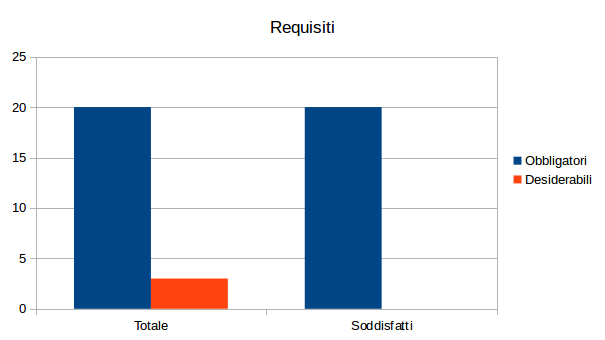
\includegraphics[scale=0.62]{immagini/graficorequisiti}
\caption{Riassunto requisiti}
\label{fig:client-server}
\end{figure}
\\I requisiti non soddisfatti riguardano direttamente gli obiettivi (e quindi non ho raggiunto) di implementazione di algoritmi di \emph{clustering} e di implementazione di algoritmi per l'individuazione dei gusti dell'utente. Tuttavia quest'ultimo obbiettivo l'ho centrato grazie all'implementazione di ID3 per fornire una raccomandazione sulla base del comportamento utente. Infine in questa attività ho soddisfatto l'obbiettivo minimo riguardante l'utilizzo di OrientDb.
\subsection{Obiettivi personali}
All'inizio dello stage il mio obbiettivo era quello di imparare nuove tecnologie da aggiungere alle mie conoscenze perché ritenevo il mio bagaglio personale insufficiente per affrontare il mondo del lavoro. Questo obbiettivo è stato certamente raggiunto, infatti lo stage mi ha permesso di padroneggiare ad un buon livello tecnologie quali OrientDb, web framework di concezione moderna e Scala. Quest'ultimo mi ha dato la possibilità di apprendere le nozioni per un corretto stile di programmazione funzionale, che era uno degli obbiettivi prefissatomi. Ritengo l'obbiettivo riguardante l'approfondimento di argomenti quali, intelligenza artificiale e i sistemi di raccomandazione, parzialmente soddisfatto. Durante lo stage non ho trovato il supporto necessario per approfondire queste competenze, soprattutto per quanto riguarda i sistemi di raccomandazione visto la natura del progetto di stage.
%**************************************************************************************************




%**************************************************************************************************
\section{Bilancio formativo}
In questa sezione viene riportato le competenze acquisite durante lo stage.\\
Lo stage in Nextep Srl è stata la  mia prima esperienza nel settore informatico, mi ha permesso di apprendere nuove competenze e consolidare competenze già apprese durante il corso di studi. Prima avevo idee molto confuse a riguardo la mia carriera professionale, ma ora dopo lo stage posso affermare di avere aspettative più ambiziose e idee più chiare su quale cammino professionale intraprendere. Ho trovato molto positivo lavorare collaborativamente al progetto perché questo mi ha portato ad migliorare le mie capacità di \emph{team working}, una \emph{skill} molto importante nel mondo del lavoro soprattutto nei contesti lavorativi dove si utilizza una metodologie \emph{agile}. Ho migliorato le mie capacità di gestione di progetto per concludere il progetto nei tempi fissati e raggiungere gli obbiettivi che mi sono prefissato. In conclusione ho concluso lo stage con un bagaglio professionale più ricco e di essere in grado di farmi carico di responsabilità più importanti.
\subsubsection{Scala}
Durante lo stage ho avuto modo di apprezzare i vantaggi derivanti dall'uso di questo linguaggio. Ho utilizzato questa tecnologia nelle attività di \emph{porting} del modulo DRE e nell'attività di sviluppo di Tres. Per studiare Scala ho seguito un corso online\footcite{https://www.coursera.org/course/progfun} tenuto direttamente dal professore Martin Odersky\footcite{http://lampwww.epfl.ch/~odersky/}, ovvero il designer del linguaggio stesso. Un corso validissimo per capirne i meccanismi e le peculiarità di questo linguaggio. All'inizio è stato un po' ostico mettere in pratica quanto appreso, ma quando ho cominciato a padroneggiare Scala ho potuto constatare un aumento della mia produttività. Mi ritengo soddisfatto di aver imparato questa tecnologia e di poter reinvestire nel mondo del lavoro questa conoscenza. 
\subsubsection{Programmazione funzionale}

\subsubsection{OrientDb}
\subsubsection{Play Framework}
%**************************************************************************************************




%**************************************************************************************************
\section{Distanza tra formazione universitaria e lavoro}
In questa sezione sezione viene esposto la valutazione personale della distanza tra la formazione ricevuta durante il corso di studi e lo stage formativo.
%**************************************************************************************************